% Tipo de documento
\documentclass[legalpaper, 12pt]{article}

% Módulos
\usepackage[utf8]{inputenc} % Codificación
\usepackage[spanish]{babel} % Español
\usepackage{multicol} % Multicolumnas
\usepackage{hyperref} % Vinculos
\usepackage{graphicx} % Imágenes
\usepackage[margin=1in]{geometry} % Márgenes
\usepackage{mathtools} % Símbolos especiales
\usepackage{pdfpages} % Importar PDF
\usepackage{fontspec} % Fonts

% Configuraciones
\setmainfont{Liberation Sans} % Fuente Principal
\setmonofont{Source Code Pro} % Fuente Principal
\graphicspath{ {images/} } % Directorio de imagenes
\DeclareSymbolFont{letters}{OML}{ztmcm}{m}{it} % Tipografía matemática

% Datos del documento
\title{Proyecto No. 2}
\author{Aguilar, Faustino \and Vásquez, Kevin}

% Ecuaciones de la Parte I
\def \eqa {\(e^x + x = 0\)}
\def \eqb {\(x^3 - 5x - 1 = 0\)}
\def \eqc {\(e^x - 2sin(x) = 0\)}

% Cuerpo del documento
\begin{document}
  \begin{titlepage}
    \centering
    \Large
    CRUV FIEC\\
    Análisis Numérico\\
    Proyecto No. 2\\
    \large
    \hfill\\
    Autores:
    \begin{multicols}{3}
      Faustino Aguilar\\
      2-732-727\\
      \columnbreak
      Kevin Vásquez\\
      9-736-2350\\
      \columnbreak
      Yolmarys González\\
      9-735-569\\
    \end{multicols}
    Profesora:\\
    Olga Batista\\
    \hfill\\
    1 de julio de 2016
  \end{titlepage}
  \newpage
  \tableofcontents
  \setcounter{page}{0}
  \newpage
  \begin{section}*{Introducción}
    \addcontentsline{toc}{section}{Introducción}
    El curso de Análisis Numérico nos ha permitido reconocer que las mátemáticas son una de las bases fundamentales de nuestra carrera. En este proyecto hemos utilizado diferentes métodos de análisis matemático que después de estudiarlos manualmente, procedimos en automatizados a través de programas informáticos para garantizar exactitud y rapidez en los cálculos para resolver una ecuacion o sistemas de ecuaciones.

    El código fuente de cada método se encuentra en un archivo adjunto a este documento. Compile y ejecute el archivo \texttt{metodos.c} para utilizar los métodos.
  \end{section}
  \newpage
  \begin{section}{Parte I}
    En esta primera parte nos encargaremos de la resolución numérica de ecuaciones con valores reales. Para cumplir con esa función se nos han asignado las siguiente ecuaciones, a resolver por los métodos dados en clase \textit{(Bisección, Punto fijo, Newton Raphson y Von Misses)}
    \begin{enumerate}
      \item \eqa
      \item \eqb
      \item \eqc
    \end{enumerate}
    \begin{figure}[h]
      \centering
      \includegraphics[scale=0.8]{eq1}
      \includegraphics[scale=0.8]{eq2}
      \includegraphics[scale=0.8]{eq3}
      \caption{Ecuaciones (1), (2) y (3) graficadas con Geogebra}
    \end{figure}
    \newpage
    \begin{subsection}{Método de Bisección de Bolsano}
      \begin{subsubsection}{Marco Teórico}
        Este es un método iterativo que consiste en utilizar un intervalo donde exista posibilidad de encontrar una solución donde corte al eje x, para ir reduciéndolo hasta llegar a la misma.

        El error es calculado por:
        \[\left|\frac{x_i-x_{i-1}}{x_i}\right|\]

        Según lo que hemos visto en las gráficas anteriores, para cada unos de los problemas tenemos los siguientes intervalos:
        \begin{enumerate}
          \item \eqa\newline
          [ -1, 0 ]
          \item \eqb\newline
          [ -2.5, -2 ] [ -0.5, 0 ] [ 2, 2.5 ]
          \item \eqc\newline
          [ -10, -9 ] [ -6.5, -7 ] [ -4, -3 ]
        \end{enumerate}
      \end{subsubsection}
      \begin{subsubsection}{Descripción de Variables}
        \begin{table}[h]
          \centering
          \begin{tabular}{|c c c|}
            \hline
            Nombre & Tipo & Utilidad\\
            \hline\hline
            o & entero & Opcion para escoger ecuacion \\
            i & entero & Contador \\
            iter & entero & Cantidad de iteraciones \\
            a & real & Primer valor del intervalo \\
            b & real & Segunro valor del intervalo \\
            tol & real & Tolerancia a soportar \\
            error & real & Error calculado \\
            x & real & Raiz anterior del problema \\
            xi & real & Siguiente Raiz del problema\\
            \hline
          \end{tabular}
          \caption{Método de Bisección: Variables utilizadas}
        \end{table}
      \end{subsubsection}
      \newpage
      \begin{subsubsection}{Resultados}
        \begin{enumerate}
          \item \eqa
          \begin{figure}[h]
            \centering
            \includegraphics[scale=0.75]{bisec1.png}
            \caption{iter=10, tol=0.01, a=-1, b=0}
          \end{figure}
          \item \eqb
          \begin{figure}[h]
            \centering
            \includegraphics[scale=0.75]{bisec2.png}
            \caption{iter=10, tol=0.01, a=-0.5, b=0}
          \end{figure}
          \newpage
          \item \eqc
          \begin{figure}[h]
            \centering
            \includegraphics[scale=0.75]{bisec3.png}
            \caption{iter=10, tol=0.01, a=-3.5, b=0}
          \end{figure}
        \end{enumerate}
      \end{subsubsection}
      \newpage
      \begin{subsubsection}{Diagrama de Flujo}
        \begin{figure}[h]
          \centering
          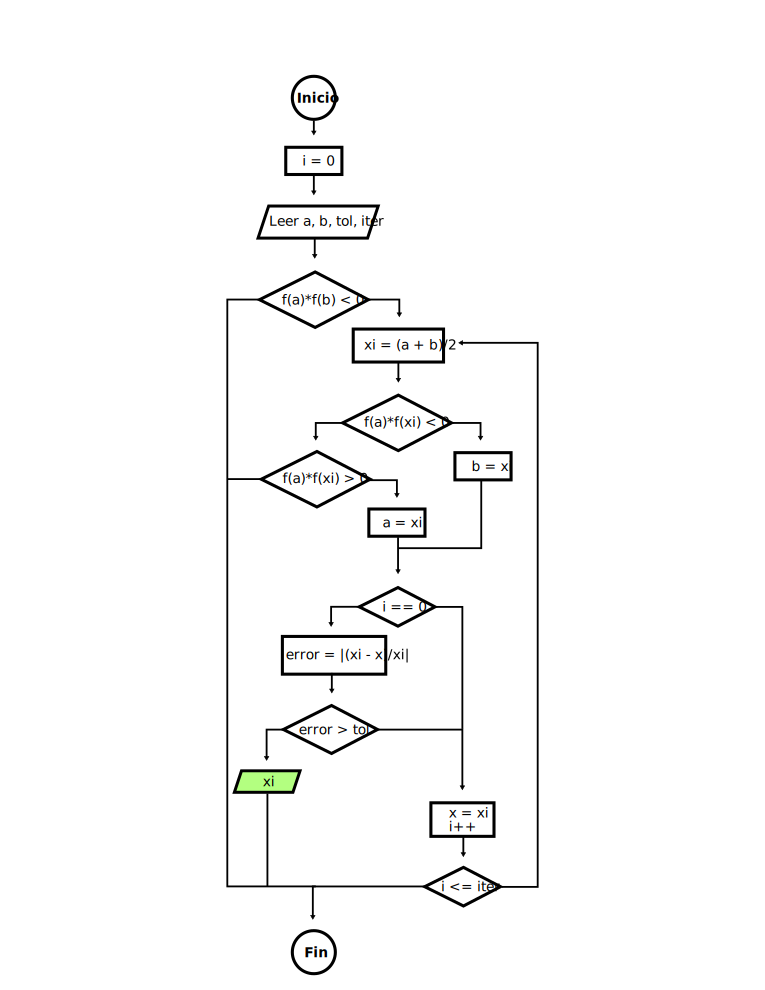
\includepdf[pages={1}]{images/biseccion.pdf}
          \caption{Diagrama de flujo del Método de Bisección}
        \end{figure}
      \end{subsubsection}
      \break
    \end{subsection}
    \break
    \begin{subsection}{Método de Punto Fijo ó Aproximaciones sucesivas}
      \begin{subsubsection}{Marco Teórico}
        Este método utiliza un algoritmo iterativo donde se utiliza una ecuación para calcular el nuevo valor y acercarse a la solución. Esta ecuación hay que encontrarla para $f(x)$, y está definida de la forma $x=g(x)$; donde $g(x)$ será nuestra ecuación de iteración siempre que $g'(x) < 1$, sino las iteraciones nunca convergerán en una solución.

        También se necesita especificar:
        \begin{enumerate}
          \item $x_0$: valor de inicio del algoritmo iterativo, lo obtenemos del estudio de la ecuación como por ejemplo el uso del método gráfico para determinar puntos cercanos a la solución.
          \item $T$: tamaño del error a tolerar, nos permite tener una solución más exacta.
          \item $n$: especifica la cantidad de veces que se ejecutará el algoritmo iterativo, debe ser de un valor razonable deacuerdo a la ecuación a resolver
        \end{enumerate}

        EL error es calculado por:
        \[\left|\frac{x_i-x_{i-1}}{x_i}\right|\]

        A continuación las ecuaciones analizadas:
        \begin{enumerate}
          \item \eqa\\$x_0=-1$\\
          Para esta ecuación podemos restar $e^x$ en ambos lados de la ecuación y nos quedaría lo siguiente:
          \[-e^x+e^x+x=-e^x\]
          \[x=-e^x\]
          \[g(x)=-e^x\]
          Derivamos $g(x)$:
          \[g'(x)=-e^x\]
          Evaluamos $x_0$ en $g'(x)$ y tenemos:
          \[g'(-1)=-e^{-1}\]
          \[g'(-1)=-0.3678794411714423\]
          Entonces $|g'(x)| < 1$ y por lo tanto podemos utilizar a $g(x)$ ya que tendrá convergencia.
          \item \eqb\\$x_0=-0.5$\\
          Para esta ecuación podemos restar $-x^3$ a ambos lados y luego dividir entre $-5$:
          \[-x^3+x^3-5x=-x^3\]
          \[\frac{-5x}{-5}=\frac{-x^3}{-5}\]
          \[x=\frac{x^3}{5}\]
          \[g(x)=\frac{x^3}{5}\]
          Derivamos $g(x)$:
          \[g'(x)=\frac{3x^2}{5}\]
          Evaluamos $x_0$ en $g'(x)$ y tenemos:
          \[g'(-0.5)=\frac{3(-0.5)^2}{5}\]
          \[g'(-0.5)=0.15\]
          Entonces $g(x)$ es una ecuación correcta porque $|g'(x)| < 1$.
          \item \eqc\\$x_0=-6.25$\\
          Para esta ecuación podemos adicionar $x$ en ambos lados:
          \[e^x -2sin(x) +x = x\]
          \[g(x) = e^x - 2sin(x) +x\]
          Derivamos $g(x)$:
          \[g'(x) = e^x-2cos(x)+1\]
          Evaluamos $x_0$ en $g'(x)$ y tenemos:
          \[g'(-6.55) = 2cos(-6.55)-e^{-6.55}+1\]
          \[g'(-6.55) = 0.9969683823127711\]
          Entonces $g(x)$ es una ecuación correcta porque $|g'(x)| < 1$.
        \end{enumerate}
      \end{subsubsection}
      \begin{subsubsection}{Descripción de Variables}
        \begin{table}[h]
          \centering
          \begin{tabular}{|c c c|}
            \hline
            Nombre & Tipo & Utilidad\\
            \hline\hline
            o & entero & Opcion para escoger ecuacion \\
            i & entero & Contador \\
            iter & entero & Cantidad de iteraciones \\
            tol & real & Tolerancia a soportar \\
            error & real & Error calculado \\
            x & real & Almacena Raiz anterior\\
            xi & real & Almacena Siguiente Raiz\\
            \hline
          \end{tabular}
          \caption{Método de Punto Fijo: Variables utilizadas}
        \end{table}
      \end{subsubsection}
      \newpage
      \begin{subsubsection}{Resultados}
        \begin{enumerate}
          \item \eqa
          \begin{figure}[h]
            \centering
            \includegraphics[scale=0.72]{pto1.png}
            \caption{iter=10, tol=0.01, x=-1}
          \end{figure}
          \item \eqb
          \begin{figure}[h]
            \centering
            \includegraphics[scale=0.72]{pto2.png}
            \caption{iter=10, tol=0.01, x=-0.5}
          \end{figure}
          \newpage
          \item \eqc
          \begin{figure}[h]
            \centering
            \includegraphics[scale=0.8]{pto3.png}
            \caption{iter=10, tol=0.01, x=-6.25}
          \end{figure}
        \end{enumerate}
      \end{subsubsection}
      \newpage
      \begin{subsubsection}{Diagrama de Flujo}
        \begin{figure}[h]
          \centering
          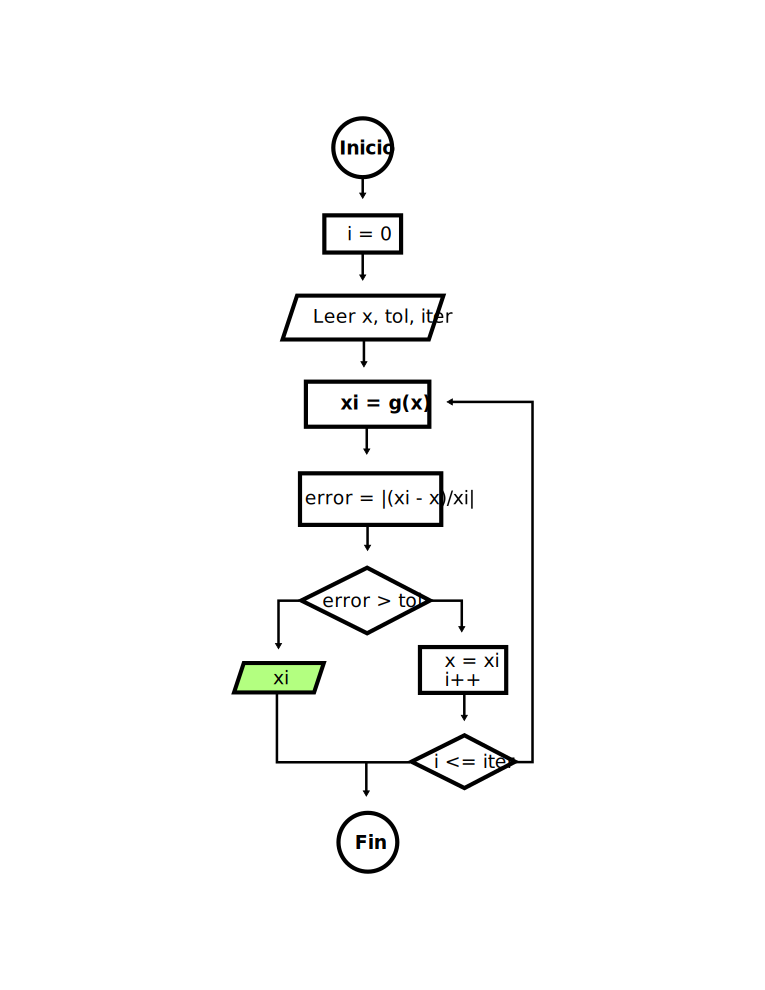
\includepdf[pages={1}]{images/punto_fijo.pdf}
          \caption{Diagrama de flujo del Método de Punto Fijo}
        \end{figure}
      \end{subsubsection}
      \break
    \end{subsection}
    \newpage
    \begin{subsection}{Método de Newton Raphson}
      \begin{subsubsection}{Marco Teórico}
        Al igual que el método anterior, este método consiste en un algoritmo iterativo, también requiere de un valor inicial $(x_0)$, tolerancia$(T)$ y número de iteraciones $(n)$. La diferencia es que el nuevo valor a calcular está dado por por:
        \[x_{i+1} = x_i - \frac{f(x_i)}{f'(x_i)}\]
        EL error es calculado por:
        \[\left|\frac{x_i-x_{i-1}}{x_i}\right|\]
        Luego para cada ecuación de la Parte I tenemos:
        \begin{enumerate}
          \item \eqa\\$x_0=-1$\\
          $f(x) = e^x+x$\\
          $f'(x) = e^x+1$
          \item \eqb\\$x_0=-0.5$\\
          $f(x) = x^3-5x$\\
          $f'(x) = 3x^2-5$
          \item \eqc\\$x_0=-3.5$\\
          $f(x) = e^x-2sin(x)$\\
          $f'(x) = e^x-2cos(x)$
        \end{enumerate}
      \end{subsubsection}
      \begin{subsubsection}{Descripción de Variables}
        \begin{table}[h]
          \centering
          \begin{tabular}{|c c c|}
            \hline
            Nombre & Tipo & Utilidad\\
            \hline\hline
            o & entero & Opcion para escoger ecuacion \\
            i & entero & Contador \\
            iter & entero & Cantidad de iteraciones \\
            tol & real & Tolerancia a soportar \\
            error & real & Error calculado \\
            x & real & Almacena Raiz anterior\\
            xi & real & Almacena Siguiente Raiz\\
            \hline
          \end{tabular}
          \caption{Método de Newton-Raphson: Variables utilizadas}
        \end{table}
      \end{subsubsection}
      \newpage
      \begin{subsubsection}{Resultados}
        \begin{enumerate}
          \item \eqa
          \begin{figure}[h]
            \centering
            \includegraphics[scale=0.8]{new1.png}
            \caption{iter=10, tol=0.01, x=-1}
          \end{figure}
          \item \eqb
          \begin{figure}[h]
            \centering
            \includegraphics[scale=0.8]{new2.png}
            \caption{iter=10, tol=0.01, x=-0.5}
          \end{figure}
          \newpage
          \item \eqc
          \begin{figure}[h]
            \centering
            \includegraphics[scale=0.8]{new3.png}
            \caption{iter=10, tol=0.01, x=-3.5}
          \end{figure}
        \end{enumerate}
      \end{subsubsection}
      \newpage
      \begin{subsubsection}{Diagrama de Flujo}
        \begin{figure}[h]
          \centering
          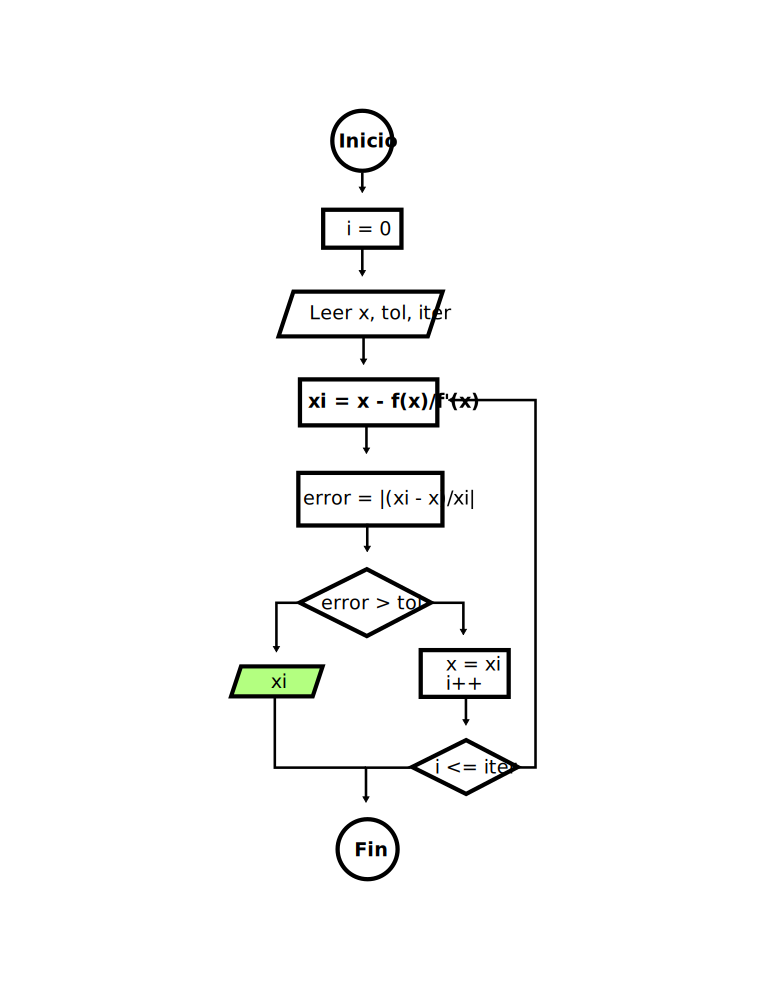
\includepdf[pages={1}]{images/newton_raphson.pdf}
          \caption{Diagrama de flujo del Método de Newton-Raphson}
        \end{figure}
      \end{subsubsection}
      \break
    \end{subsection}
    \newpage
    \begin{subsection}{Método de Von Misses}
      \begin{subsubsection}{Marco Teórico}
        Este método también consiste en un algoritmo iterativo, y es muy parecido al método de Newton Raphson, también requiere de un valor inicial $(x_0)$, tolerancia$(T)$ y número de iteraciones $(n)$. La diferencia es que el nuevo valor a calcular está dado por por:
        \[x_{i+1} = x_i - \frac{f(x_i)}{f'(x_0)}\]

        El denominador siempre es $f'(x_0)$, entonces para cada ecuación de la Parte I tenemos:
        \begin{enumerate}
          \item \eqa\\$x_0=-1$\\
          $f(x) = e^x+x$\\
          $f'(x_0) = e^x+1$\\
          $f'(-1) = 1.367879441171442$
          \item \eqb\\$x_0=-0.5$\\
          $f(x) = x^3-5x$\\
          $f'(x_0) = 3x^2-5$\\
          $f'(-0.5) = -4.25$
          \item \eqc\\$x_0=-3.5$\\
          $f(x) = e^x-2sin(x)$\\
          $f'(x_0) = e^x-2cos(x)$\\
          $f'(-3.5) = 1.903110758003911$
        \end{enumerate}

        Podemos asignar el valor de $f'(x_0)$ a una variable que no cambia.
      \end{subsubsection}
      \begin{subsubsection}{Descripción de Variables}
        \begin{table}[h]
          \centering
          \begin{tabular}{|c c c|}
            \hline
            Nombre & Tipo & Utilidad\\
            \hline\hline
            o & entero & opcion para escoger ecuacion \\
            i & entero & contador \\
            iter & entero & cantidad de iteraciones \\
            tol & real & tolerancia a soportar \\
            error & real & error calculado \\
            x0 & real & Almacena Primera raiz\\
            x & real & Almacena Raiz anterior\\
            xi & real & Almacena Siguiente Raiz\\
            f & real & Almacena el resultado de f(x)\\
            F & real & Almacena el resultado de f'(x)\\
            \hline
          \end{tabular}
          \caption{Método de Von-Misses: Variables utilizadas}
        \end{table}
      \end{subsubsection}
      \newpage
      \begin{subsubsection}{Resultados}
        \begin{enumerate}
          \item \eqa
          \begin{figure}[h]
            \centering
            \includegraphics[scale=0.8]{von1.png}
            \caption{iter=10, tol=0.01, x=-1}
          \end{figure}
          \item \eqb
          \begin{figure}[h]
            \centering
            \includegraphics[scale=0.8]{von2.png}
            \caption{iter=10, tol=0.01, x=-0.5}
          \end{figure}
          \newpage
          \item \eqc
          \begin{figure}[h]
            \centering
            \includegraphics[scale=0.8]{von3.png}
            \caption{iter=10, tol=0.01, x=-3.5}
          \end{figure}
        \end{enumerate}
      \end{subsubsection}
      \newpage
      \begin{subsubsection}{Diagrama de Flujo}
        \begin{figure}[h]
          \centering
          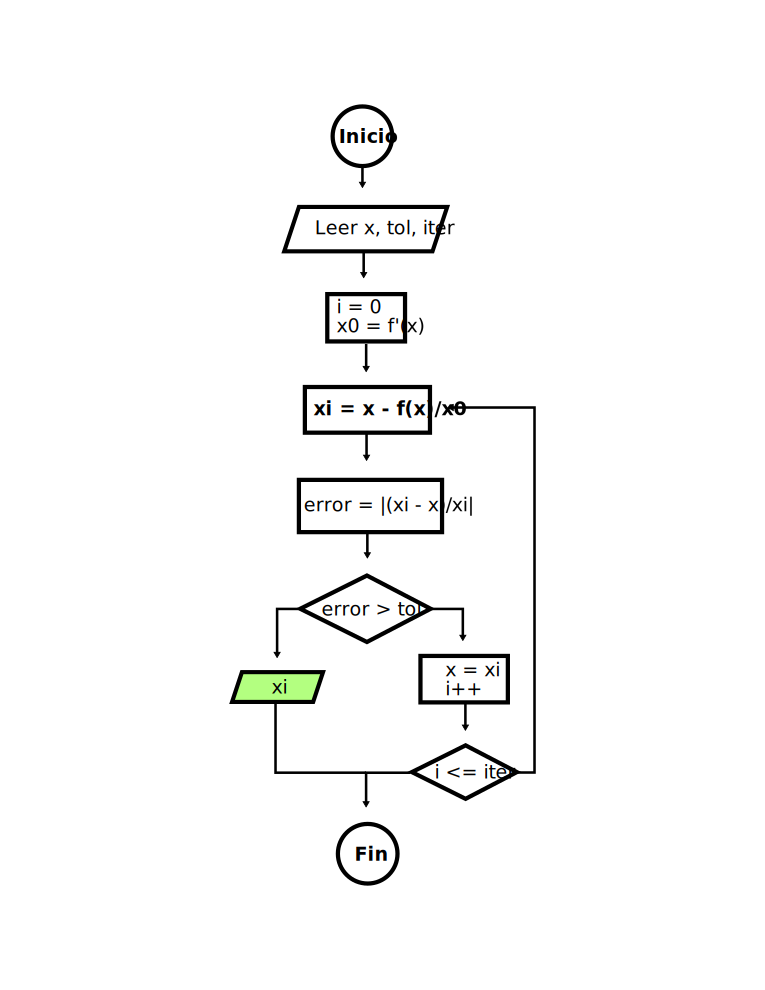
\includepdf[pages={1}]{images/von_misses.pdf}
          \caption{Diagrama de flujo del Método de Von-Misses}
        \end{figure}
      \end{subsubsection}
      \break
    \end{subsection}
    \begin{subsection}{Conclusiones}
      \begin{description}
        \item[\eqa:] Esta fue la ecuación más simple de todas, puedo
        ser resuelta sin problemas en todos los metodos de la Parte 1, sin embargo
        podemos recalcar que se ejecutó con mayor rapidez en el método de Newton-Raphson.
        \item[\eqb:] Esta ecuación al ser análizada logramos observar que tenía
        tres soluciones o raices posibles, por lo que nos dio algunos problemas
        ya que se necesitaba elegir los valores correctos para resolverla,
        viendo que en Método de Bisección en la utilización de intervalos fue la más
        sencilla y factible.
        \item[\eqc:] Esta fue la ecuación más complicada de todas, especialmente en
        el método de Punto Fijo ya que nos fijamos que la g(x) solo funcionaba con
        valores muy cercanos a la solución, dificultando su análisis. Sin embargo
        por los otros Métodos si se pudo resolver sin mayor inconveniente, utilizando
        en el caso de bisección los intervalos y cuando era Newton-Raphson y Von-Misses
        la derivada de f(x).
      \end{description}
    \end{subsection}
  \end{section}
  \newpage
  \begin{section}{Parte II}
    Resolución numérica de sistemas de ecuaciones algebraicas
    simultáneas con valores reales.
    \begin{subsection}{Método de Gauss}
      \begin{subsubsection}{Marco Teórico}
        El método de Gauss consiste en transformar un sistema de ecuaciones
        en otro equivalente de forma que este sea escalonado.
        Para facilitar el cálculo vemos el sistema como una matriz,
        en la que pondremos los coeficientes de las variables y los términos
        independientes (separados por una recta).

        Es una generalización del método de reducción, que utilizamos para eliminar
        una incógnita en los sistemas de dos ecuaciones con dos incógnitas.
        Consiste en la aplicación sucesiva del método de reducción, utilizando los
        criterios de equivalencia de sistemas, para transformar la matriz ampliada
        con los términos independientes en una matriz triangular, de modo que cada
        fila (ecuación) tenga una incógnita menos que la inmediatamente anterior.
        Se obtiene así un sistema, que llamaremos escalonado, tal que la última
        ecuación tiene una única incógnita, la penúltima dos incógnitas,
        la antepenúltima tres incógnitas y la primera todas las incógnitas.
      \end{subsubsection}
      \begin{subsubsection}{Descripción de Variables}
        \begin{table}[h]
          \centering
          \begin{tabular}{|c c c|}
            \hline
            Nombre & Tipo & Utilidad\\
            \hline\hline
            n & entero & Tamaño de la matriz NxN\\
            i & entero & Contador \\
            j & entero & Contador \\
            k & entero & Contador \\
            mayor & entero & Mayor número de fila \\
            aux & real & Variable temporal para guardar resultados \\
            m[N][N] & real & Matriz idéntica a resolver \\
            x[N] & real & Soluciones del sistema de ecuaciones \\
            \hline
          \end{tabular}
          \caption{Método de Gauss: Variables utilizadas}
        \end{table}
      \end{subsubsection}
      \newpage
      \begin{subsubsection}{Resultados}
        El sistema de ecuaciones para resolver en el programa es:
        \[x+y+z+u=10\]
        \[2x-y+3z-4u=9\]
        \[3x+2y-z+5u=13\]
        \[x-3y+2z-4u=-3\]

        Este sistema de ecuaciones el uno de los que se propuso en la hoja
        del Proyecto.
        \begin{figure}[h]
          \centering
          \includegraphics[scale=0.9]{gauss.png}
          \caption{Eliminacion de Gauss}
        \end{figure}
      \end{subsubsection}
      \newpage
      \begin{subsubsection}{Diagrama de Flujo}
        \begin{figure}[h]
          \centering
          \includepdf[pages={1}]{images/gauss.pdf}
          \caption{Diagrama de flujo del Método de Eliminación de Gauss}
        \end{figure}
      \end{subsubsection}
      \break
    \end{subsection}
    \break
    \begin{subsection}{Método de Gauss Jordan}
      \begin{subsubsection}{Marco Teórico}
        Es un algoritmo del álgebra lineal para determinar las soluciones
        de un sistema de ecuaciones lineales, encontrar matrices e inversas.
        Un sistema de ecuaciones se resuelve por el método de Gauss cuando se
        obtienen sus soluciones mediante la reducción del sistema dado a otro
        equivalente en el que cada ecuación tiene una incógnita menos que la anterior.
        El método de Gauss transforma la matriz de coeficientes en una matriz
        triangular superior. El método de Gauss-Jordan continúa el proceso de
        transformación hasta obtener una matriz diagonal.
      \end{subsubsection}
      \begin{subsubsection}{Descripción de Variables}
        \begin{table}[h]
          \centering
          \begin{tabular}{|c c c|}
            \hline
            Nombre & Tipo & Utilidad\\
            \hline\hline
            n & entero & Tamaño de la matriz NxN\\
            i & entero & Contador \\
            j & entero & Contador \\
            k & entero & Contador \\
            mayor & entero & Mayor número de fila \\
            aux & real & Variable temporal para guardar resultados \\
            pivote & real & Elemento en la posición m[i][i] \\
            m[N][N] & real & Matriz idéntica a resolver \\
            x[N] & real & Soluciones del sistema de ecuaciones \\
            \hline
          \end{tabular}
          \caption{Método de Gauss-Jordan: Variables utilizadas}
        \end{table}
      \end{subsubsection}
      \newpage
      \begin{subsubsection}{Resultados}
        El sistema de ecuaciones para resolver en el programa es:
        \[x+y+z+u=10\]
        \[2x-y+3z-4u=9\]
        \[3x+2y-z+5u=13\]
        \[x-3y+2z-4u=-3\]
        \begin{figure}[h]
          \centering
          \includegraphics[scale=0.9]{jordan.png}
          \caption{Matriz idéntica de Gauss-Jordan}
        \end{figure}
      \end{subsubsection}
      \newpage
      \begin{subsubsection}{Diagrama de Flujo}
        \begin{figure}[h]
          \centering
          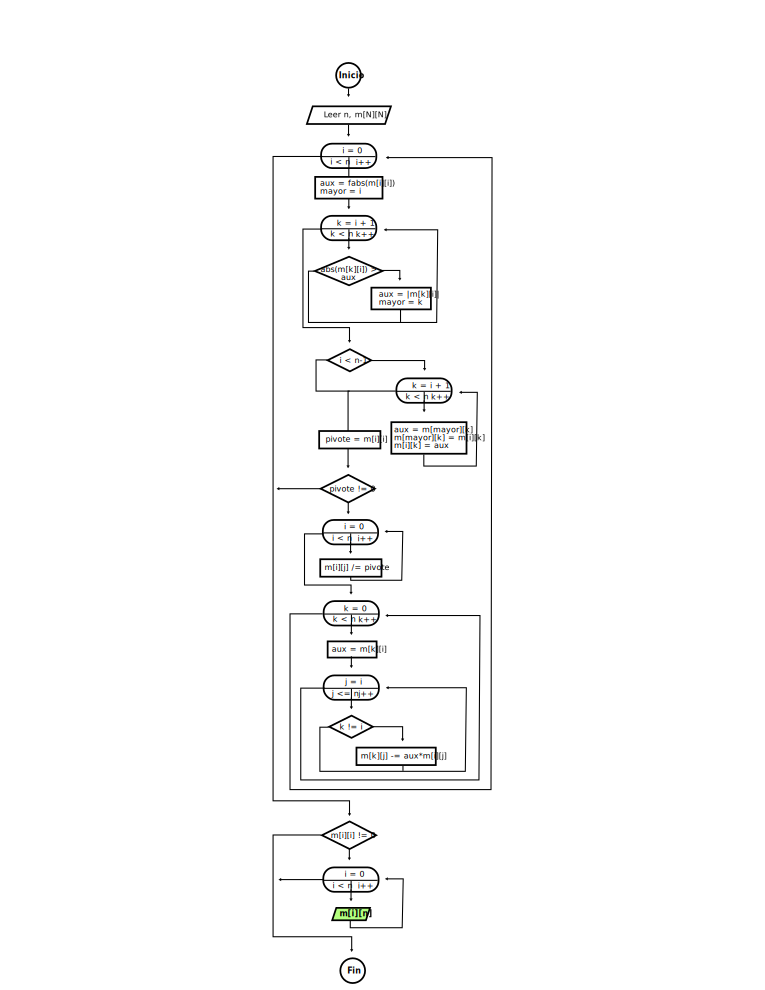
\includepdf[pages={1}]{images/gauss_jordan.pdf}
          \caption{Diagrama de flujo del Método de Gauss-Jordan}
        \end{figure}
      \end{subsubsection}
      \break
    \end{subsection}
    \begin{subsection}{Método de Jacobi}
      \begin{subsubsection}{Marco Teórico}
        Es un método iterativo, usado para resolver sistemas de ecuaciones
        lineales del tipo $Ax = b$
        La base del método consiste en construir una sucesión convergente
        definida iterativamente. El límite de esta sucesión es precisamente
        la solución del sistema. A efectos prácticos si el algoritmo se detiene
        después de un número finito de pasos se llega a una aproximación al valor
        de x de la solución del sistema.

        El error se calcula de la siguiente manera:
        
        Se conoce como la norma de $\frac{Xi - X}{Xi}$

        \[D_1 = sqrt((x_i-x_{i-1})^2)\]
        \[D_2 = sqrt((x_i)^2)\]
        \[E = \frac{D_1}{D_2}\]

      \end{subsubsection}
      \begin{subsubsection}{Descripción de Variables}
        \begin{table}[h]
          \centering
          \begin{tabular}{|c c c|}
            \hline
            Nombre & Tipo & Utilidad\\
            \hline\hline
            n & entero & Tamaño de la matriz NxN\\
            i & entero & Contador \\
            j & entero & Contador \\
            aux[i] & real & Variable temporal para guardar resultados\\
            pivote & real & Elemento en la posición m[i][i] \\
            x[N] & real & Aprox. del sistema de ecuaciones \\
            xi[N] & real & Aprox. siguientes del sistema de ecuaciones \\
            coef[N][N] & real & Coeficientes del sistema de ecuaciones \\
            l[N] & real & Términos libres del sistema de ecuaciones \\
            d1 & real & Dividendo para el calculo del error\\
            d2 & real & Divisor para el calculo del error\\
            tol & real & Tolerancia aceptada\\
            error & real & Error calculado con d1 y d2\\
            \hline
          \end{tabular}
          \caption{Método de Jacobi: Variables utilizadas}
        \end{table}
      \end{subsubsection}
      \newpage
      \begin{subsubsection}{Resultados}
        El sistema de ecuaciones para resolver en el programa es:
        \[10x_1-x_2=9\]
        \[-x_1+10x_2-2x_3=7\]
        \[-2x_2+10x_3=6\]

        Este sistema fue desarrollado en el Parcial 2 de Análisis Numérico,
        se utilizaron los siguientes datos:
        \begin{description}
          \item[Tolerancia=]0.01
          \item[Iteraciones=]10
          \item[Valore iniciales=](0,0,0)
        \end{description}
        \begin{figure}[h]
          \centering
          \includegraphics[scale=0.9]{jacobi.png}
          \caption{Resultado de Jacobi}
        \end{figure}
      \end{subsubsection}
      \newpage
      \begin{subsubsection}{Diagrama de Flujo}
        \begin{figure}[h]
          \centering
          \includepdf[pages={1}]{images/jacobi.pdf}
          \caption{Diagrama de flujo del Método de Jacobi}
        \end{figure}
      \end{subsubsection}
      \break
    \end{subsection}
    \begin{subsection}{Método de Gauss Seidel}
      \begin{subsubsection}{Marco Teórico}
        El método de Gauss-Seidel es un método iterativo utilizado para resolver
        sistemas de ecuaciones lineales. Es un método iterativo, lo que significa
        que se parte de una aproximación inicial y se repite el proceso hasta
        llegar a una solución con un margen de error tan pequeño como se quiera.

        En este método a diferencia de Jacobi, se utilizan los valores de x una
        vez son generados sin esperar otra iteracion.

        EL error se calcula de la misma manera:

        \[D_1 = sqrt((x_i-x_{i-1})^2)\]
        \[D_2 = sqrt((x_i)^2)\]
        \[E = \frac{D_1}{D_2}\]
      \end{subsubsection}
      \begin{subsubsection}{Descripción de Variables}
        \begin{table}[h]
          \centering
          \begin{tabular}{|c c c|}
            \hline
            Nombre & Tipo & Utilidad\\
            \hline\hline
            n & entero & Tamaño de la matriz NxN\\
            i & entero & Contador \\
            j & entero & Contador \\
            aux & real & Variable temporal para guardar resultados\\
            pivote & real & Elemento en la posición m[i][i] \\
            x[N] & real & Aprox. del sistema de ecuaciones \\
            xi[N] & real & Aprox. siguientes del sistema de ecuaciones \\
            coef[N][N] & real & Coeficientes del sistema de ecuaciones \\
            l[N] & real & Términos libres del sistema de ecuaciones \\
            d1 & real & Dividendo para el calculo del error\\
            d2 & real & Divisor para el calculo del error\\
            tol & real & Tolerancia aceptada\\
            error & real & Error calculado con d1 y d2\\
            \hline
          \end{tabular}
          \caption{Método de Gauss-Seidel: Variables utilizadas}
        \end{table}
      \end{subsubsection}
      \newpage
      \begin{subsubsection}{Resultados}
        El sistema de ecuaciones para resolver en el programa es:
        \[10x_1-x_2=9\]
        \[-x_1+10x_2-2x_3=7\]
        \[-2x_2+10x_3=6\]

        Este sistema fue desarrollado en el Parcial 2 de Análisis Numérico,
        se utilizaron los siguientes datos:
        \begin{description}
          \item[Tolerancia=]0.01
          \item[Iteraciones=]10
          \item[Valore iniciales=](0,0,0)
        \end{description}
        \begin{figure}[h]
          \centering
          \includegraphics[scale=0.9]{seidel.png}
          \caption{Resultado de Gauss-Seidel}
        \end{figure}
      \end{subsubsection}
      \newpage
      \begin{subsubsection}{Diagrama de Flujo}
        \begin{figure}[h]
          \centering
          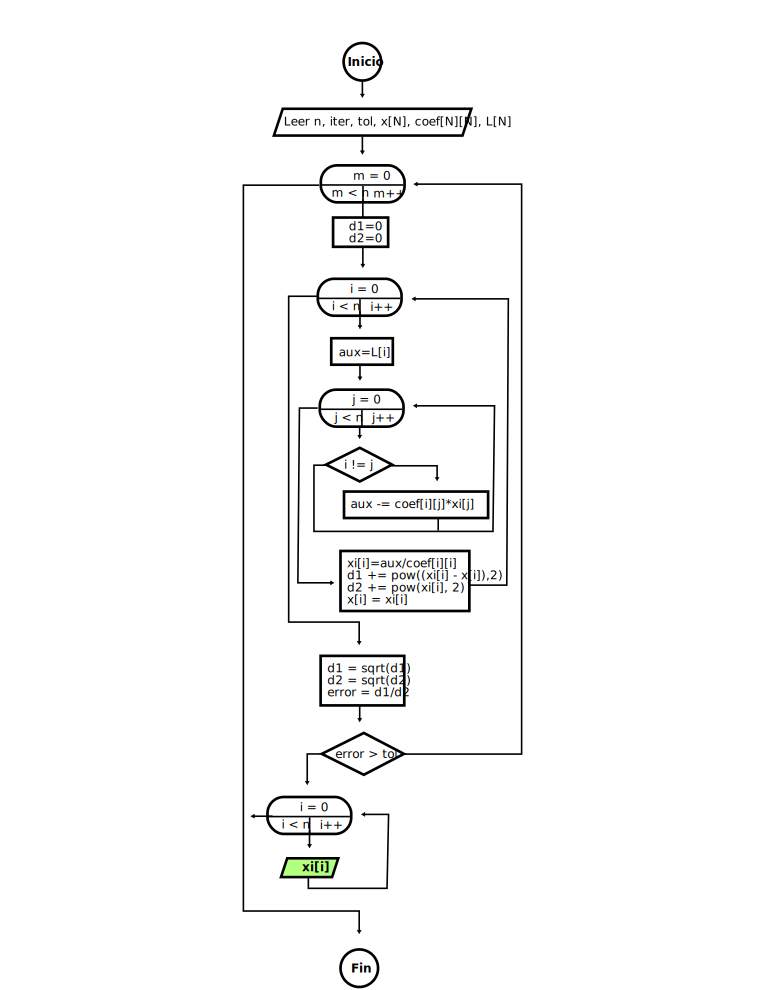
\includepdf[pages={1}]{images/gauss_seidel.pdf}
          \caption{Diagrama de flujo del Método de Gauss-Seidel}
        \end{figure}
      \end{subsubsection}
      \break
    \end{subsection}
    \begin{subsection}{Conclusiones}
      Se dio la resolución
      Al desarrollar los métodos de solucion numérica de sistema de
      ecuaciones algebraicas, logramos hacer que nuestro programa
      funcionara para resolver ecuaciones por cualquiera de los métodos,
      siendo algunos más exactos que otros.

      En cuanto a la análisis del los métodos podemos concluir que:
      \begin{itemize}
        \item \textbf{Método de Gauss:} Ha sido un método que se ve más
        sencillo al principio pero que resulta en mayor grado de complicación
        cuando se tiene que buscar las raices regresivamente.
        \item \textbf{Método de Gauss-Jordan:} Para nosotros es considerado el más
        factible de todos, ya que al completar la matriz identica encontramos el
        resultado, sin tener que hacer nada más.
        \item \textbf{Método de Jacobi:} Este es un método iterativo, que nos
        resulto con más dificultad de implementación, que los métodos anteriores
        principalmente porque hay más datos de entrada y el error se calcula
        de una manera más complicada.
        \item \textbf{Método de Gauss-Seidel:} En nuestras pruebas logramos, entender
        que era casi lo mismo que el método de Jacobi, la única diferencia es que
        aqui se utiliza el valor de x de inmediato cuando es generado y no se
        espera a la siguiente iteracion como lo hace Jacobi, resultando que
        en algunos problemas se den menos iteraciones.
      \end{itemize}
    \end{subsection}
  \end{section}
  \newpage
  \nocite{*}
  \begin{bibliography}{bibliografia}
    \bibliographystyle{apalike}
    \addcontentsline{toc}{section}{Referencias}
  \end{bibliography}
\end{document}
